\section{Аналитическое исследование\\поставленной задачи}

\subsection{Теорема о неустойчисвости приближений\\старших порядков}\label{sec:conidtions}

Напомним, что в настоящей работе исследуется задача

\begin{equation}
\left\{
\begin{aligned}
\rho_t(\bar{x},t) + div \bar{J}(\bar{x},t) = f(\bar{x},t),\\
\bar{J}(\bar{x},t+\tau) = -a^2 \nabla \rho(\bar{x},t) + \bar{V}(\bar{x},t) \rho(\bar{x},t)
\end{aligned}
\right.
\end{equation}

Для нее в условиях

\begin{enumerate}\label{eq:init-modelled}
\item одномерной задачи,
\item $\rho (x,t) = e^{\frac{V}{2a^2} x} u(x,t)$,
\item $\sum\limits_{n=0}^{m} \dfrac{\partial^n f}{\partial t^n} \dfrac{\tau^n}{n!} = g(x,t) \equiv 0 \Leftarrow f(x,t) \equiv 0$,
\item $V=const$
\end{enumerate}

были построены приближения

\begin{equation}\label{eq:transfer-modelled}
\sum\limits_{n=0}^{m} \dfrac{\partial^{n+1} u}{\partial t^{n+1}} \dfrac{\tau^n}{n!} - a^2 \dfrac{\partial^2 u}{\partial x^2} + \dfrac{V^2}{4a^2} u = 0,
\end{equation}

решения которых устойчивы при устойчивости решений обыкновенного дифференциального уравнения

\begin{equation}\label{eq:ODE-modelled}
\sum\limits_{n=0}^{m} \dfrac{\tau^n}{n!} T^{(n+1)} + \underbrace{ \left( \dfrac{V^2}{4a^2} + a^2 k^2 \right)}_{\gamma(k^2)} T = 0
\end{equation}

и неустойчивы в противном случае.

При анализе результатов моделирования было выдвинуто предположение о неустойчивости всех приближений, начиная с $m=6$.

\so{\textbf{Теорема о неустойчивости приближений\\старших порядков}}. Приближения (\ref{eq:transfer-modelled}) задачи (\ref{eq:init-modelled}) всех порядков кроме $m=1$ неустойчивы.

Для доказательства теоремы сначала докажем следующее утверждение:

\so{\textbf{Утверждение}}. $\Delta_3 < 0$ при $m \geq 6$.

Выпишем общий вид определителя матрицы Гурвица при $k=3$:

\begin{equation*}
\Delta_3 = 
\begin{vmatrix}
\frac{\tau^{m-1}}{(m-1)!} & \frac{\tau^{m}}{m!} & 0\\
\frac{\tau^{m-3}}{(m-3)!} & \frac{\tau^{m-2}}{(m-2)!} & \frac{\tau^{m-1}}{(m-1)!}\\
\frac{\tau^{m-5}}{(m-5)!} & \frac{\tau^{m-4}}{(m-4)!} & \frac{\tau^{m-3}}{(m-3)!}
\end{vmatrix} =
\dfrac{\tau^{m-1}}{(m-1)!}
\begin{vmatrix}
\frac{\tau^{m-2}}{(m-2)!} & \frac{\tau^{m-1}}{(m-1)!}\\
\frac{\tau^{m-4}}{(m-4)!} & \frac{\tau^{m-3}}{(m-3)!}
\end{vmatrix}
- \dfrac{\tau^{m}}{m!}
\begin{vmatrix}
\frac{\tau^{m-3}}{(m-3)!} & \frac{\tau^{m-1}}{(m-1)!}\\
\frac{\tau^{m-5}}{(m-5)!} & \frac{\tau^{m-3}}{(m-3)!}
\end{vmatrix}
\end{equation*}

\begin{equation*}
\Delta_3 =
\dfrac{\tau^{m-1}}{(m-1)!} \dfrac{\tau^{m-2}}{(m-2)!} \dfrac{\tau^{m-4}}{(m-4)!}
\begin{vmatrix}
1 & \frac{\tau}{m-1}\\
1 & \frac{\tau}{m-3}
\end{vmatrix}
- \dfrac{\tau^{m}}{m!} \dfrac{\tau^{m-3}}{(m-3)!} \dfrac{\tau^{m-5}}{(m-5)!}
\begin{vmatrix}
1 & \frac{\tau^2}{(m-2)(m-1)}\\
1 & \frac{\tau^2}{(m-4)(m-3)}
\end{vmatrix}
\end{equation*}

\begin{multline*}
\Delta_3 = \dfrac{\tau^{3m-7}}{(m-1)!(m-2)!(m-4)!} \left( \dfrac{\tau}{m-3} - \dfrac{\tau}{m-1} \right) \\ - \dfrac{\tau^{3m-8}}{m!(m-3)!(m-5)!} \left( \dfrac{\tau^2}{(m-4)(m-3)} - \dfrac{\tau^2}{(m-2)(m-1)} \right)
\end{multline*}

\begin{multline*}
\Delta_3 = \tau^{3m-6} \left( \dfrac{(m-1) - (m-3)}{(m-1)!(m-2)!(m-4)!(m-3)(m-1))} \right. \\ \left. - \dfrac{(m-2)(m-1) - (m-4)(m-3)}{m!(m-3)!(m-5)!(m-4)(m-3)(m-2)(m-1)} \right)
\end{multline*}

\begin{align*}
\Delta_3 = \dfrac{\tau^{3m-6}}{m!(m-1)!(m-3)!} (2m - (-3m + 2 + 7m - 12)) =\\= \dfrac{\tau^{3m-6}}{m!(m-1)!(m-3)!} (10-2m) < 0
\end{align*}

при $m \geq 6$.

Таким образом, осталось доказать неустойчивость нулевого решения \ref{eq:ODE-modelled} при $1 \leq m \leq 5$ в предположениях достаточно больших значений $\gamma(k^2)$ и ограниченности $\tau$.

\textbf{при $m=1$}: $\Delta_1 = 1 > 0$, $\Delta_1 = \gamma > 0$\\

\textbf{при $m=2$}: $\Delta_1 = \tau > 0$, $\Delta_2 = \tau (1 - \frac{1}{2} \gamma \tau) < 0$, $\Delta_3 = \gamma \tau (1 - \frac{1}{2} \gamma \tau) < 0$\\

\textbf{при $m=3$}: $\Delta_1 = \frac{1}{2} \tau ^2 > 0$, $\Delta_2 = \frac{1}{3} \tau ^3 > 0$, $\Delta_3 = \tau ^3 (\frac{1}{3} - \frac{1}{4} \gamma  \tau ) < 0$, $\Delta_4 = \gamma  \tau ^3 (\frac{1}{3} - \frac{1}{4} \gamma  \tau ) < 0$\\

\textbf{при $m=4$}: $\Delta_1 = \frac{1}{6} \tau ^3 > 0$, $\Delta_2 = \frac{1}{24} \tau ^5 > 0$, $\Delta_3 = \frac{1}{144} \tau^6 (2+\gamma \tau) > 0$, $\Delta_4 = \frac{1}{576} \tau^6 (8 - 4 \gamma \tau - \gamma^2 \tau^2 ) < 0$, $\Delta_5 = \frac{1}{576} \gamma \tau^6 (8 - 4 \gamma \tau - \gamma^2 \tau^2 < 0)$\\

\textbf{при $m=5$}: $\Delta_1 = \frac{1}{24} \tau^4 > 0$, $\Delta_2 = \frac{1}{360} \tau^7 > 0$, $\Delta_3 = 0$,\\$\Delta_4 = \frac{1}{14400} \tau^{10} (\frac{8}{3} + \frac{5}{3} \gamma \tau) > 0$, $\Delta_5 = \frac{1}{14400} \tau^{10} (-\frac{8}{3} + \frac{10}{3} \gamma \tau - \frac{25}{24} \gamma^2 \tau^2) < 0$, $\Delta_6 = \frac{1}{14400} \gamma \tau^{10} (-\frac{8}{3} + \frac{10}{3} \gamma \tau - \frac{25}{24} \gamma^2 \tau^2) < 0$\\

Теорема доказана.\\

Таким образом, для всех приближений кроме первого нарушается условие непрерывной зависимости решений он начальных данных в силу их неустойчивости, т.е сами приближения \--- некорректно поставленные по Адамару задачи.

\subsection{Устойчивость решений дифферециального уравненения\\с запаздыванием по времени}

Напомним, что предварительно было получен общий вид уравнения с запаздыванием \ref{eq:main-one} для исходной задачи:

\begin{equation*}
\rho_t(\bar{x},t) = -a^2 \Delta \rho(\bar{x},t-\tau) + \rho(\bar{x},t-\tau) div \bar{V}(\bar{x},t-\tau) + (\bar{V}(\bar{x},t-\tau),\nabla \rho(\bar{x},t-\tau))
\end{equation*}

В тех же условиях, для которых были получены приближения для него (они перечислены, например, в начале пункта [\ref{sec:conditions}]), можно вывести следующее:

\begin{equation}
\rho_t (x,t) - a^2 \rho_{xx} (x,t-\tau) + V \rho_x (x,t-\tau) = 0
\end{equation}

Так как подобный вывод уже был произведен в пункте [\ref{sec:transition}], опустим подробности и получим:

\begin{equation}\label{eq:diffusion-reaction-delay}
u_t (x,t) - a^2 u_{xx} (x,t-\tau) + \dfrac{V^2}{4a^2} u_x (x,t-\tau) = 0
\end{equation}

Для \ref{eq:diffusion-reaction-delay} применим метод Фурье разделения переменных

\begin{equation}
u(x,t) = \sum\limits_{k=1}^{\infty} X(x) T(t)
\end{equation}

Отметим, что, вообще говоря, метод Фурье непременим к любому дифференциальному уравнению с запаздыванием (даже линейному), но в данном случае с его помощью можно получить такие результаты:

\begin{equation}
X(x) T'(t) + \dfrac{V^2}{4a^2} X(x) T(t-\tau) =a^2 X''(x) T(t-\tau), \quad k=1,\dots,\infty
\end{equation}

\begin{equation}
\dfrac{T'(t) + \dfrac{V^2}{4a^2} T(t-\tau)}{a^2 T(t-\tau)} = \dfrac{X''(x)}{X(x)} = -\lambda = -k^2
\end{equation}

Наконец, получим:

\begin{equation}
\left\{
\begin{aligned}
T'(t) + \underbrace{ \left( \dfrac{V^2}{4a^2} + a^2 k^2 \right)}_{\gamma(k^2)} T(t-\tau) & = 0\\
X'' + k^2 X & = 0
\end{aligned}
\right.
\end{equation}

Поставим задачу Коши c постоянной начальной функцией для уравнения относительно $T(t)$:

\begin{equation}\label{eq:Cauchy-delayed}
\left\{
\begin{aligned}
T'_k (t) + \underbrace{ \left( \dfrac{V^2}{4a^2} + a^2 k^2 \right)}_{\gamma(k^2)} T_k (t-\tau) = 0, \quad t>0,\\
T_k (t) = T_{k}^{0}, \quad -\tau \leq t \leq 0.
\end{aligned}
\right.
\end{equation}

Отметим, что если в нем совершить формальный временной сдвиг на $\tau$ и применить уже используемое в настоящей работе разложение

\begin{equation}
T(t+\tau) = T(t) + \tau T'(t) + \dots + \dfrac{\tau^n}{n!} T^{(n)} (t) + \dots,
\end{equation}

то получим исходные приближения (\ref{eq:transfer-modelled}), для которых уже был исследован вопрос устойчивости.

Для решений уравнения из задачи (\ref{eq:Cauchy-delayed}) справедливо характеристическое уравнение

\begin{equation}
\lambda_k + \gamma(k^2) e^{-\lambda_k \tau} = 0
\end{equation}

Устойчивость (\ref{eq:transfer-modelled}) зависит от знаков вещественных частей $Re(\lambda_k)$.

\subsection{Достаточное условие неположительности знаков\\вещественных частей корней характерестического\\уравнения}

Напомним, что задача свелась к поиску параметров таких, что все вещественные части корней характерического уравнения

\begin{equation}
\phi(z) = z + \gamma e^{-z \tau}
\end{equation}

отрицательны.

Приведем вспомогательную теорему:

\so{\textbf{Теорема Руше}} Если комплекснозначные функции $f(z)$ и $g(z)$ голоморфны в односвязной области $G$, а на её границе $\delta G$ выполняется неравенство $|g(z)| < |f(z)|$, то $f(z)$ и $(f+g)(z)$ имеют одинаковое число нулей с учетом кратности.

Данную теорему используем в доказательстве следующего факта:

\so{\textbf{Достаточное условие отсутствия корней с положительными вещественными частями характерестического уравнения $\phi(z) = z + \gamma e^{-z \tau}$}}.

\begin{equation*}
\phi(z) = z + \gamma e^{-z \tau}
\end{equation*}

положительными вещественными частями при $\gamma \tau < 1$.

Для доказательства этого факта представим $\phi (z)$ в следующем виде:

\begin{equation}
\phi(z) = \underbrace{{z + \gamma}}_{H_1(z)} + \underbrace{z \gamma \tau \left(\dfrac{e^{-z \tau} - 1}{z \tau} \right)}_{H_2(z)} = 0
\end{equation}

Рассмотрим функции $H_1(z)$ и $H_2(z)$ в области $D = {z|Re(z) \geq 0}$. Её границей будет ось чисто мнимых чисел $\delta D = {z|Re(z)=0}$.

Отметим, что $H_1(z)>0$ в открытой области $D-\delta D$ при любом $z$.

Представим $z=x+iy$ и рассмотрим $H_1(z)$ и $H_2(z)$ в области $\delta D$ (т.е. $z=iy$):

\begin{equation}\label{eq:h1}
|H_1(iy)| = \sqrt{\gamma^2 + y^2} > |y| = |z|
\end{equation}

Представим $H_2(z)$:

\begin{equation}
H_2(z) = z \gamma \tau \underbrace{\left(\dfrac{e^{-z \tau} - 1}{z \tau} \right)}_{h(z)}
\end{equation}

\begin{equation}
h(iy) = \dfrac{cos(y \tau) - i sin(y \tau) - 1}{iy \tau} = -\dfrac{sin(y \tau)}{y \tau} - i \dfrac{cos(y \tau)-1}{y \tau}
\end{equation}

Обозначим $\alpha = y \tau$

\begin{equation}
{|h(iy)|}^2 = \dfrac{sin^2(\alpha)}{\alpha^2} + \dfrac{(cos(\alpha)-1)^2}{\alpha^2} = \dfrac{2-2cos(\alpha)}{\alpha^2} \leq 1
\end{equation}

Для наглядности приведем график ${|h(iy)|}^2$:

\begin{figure}[h]
\begin{center}
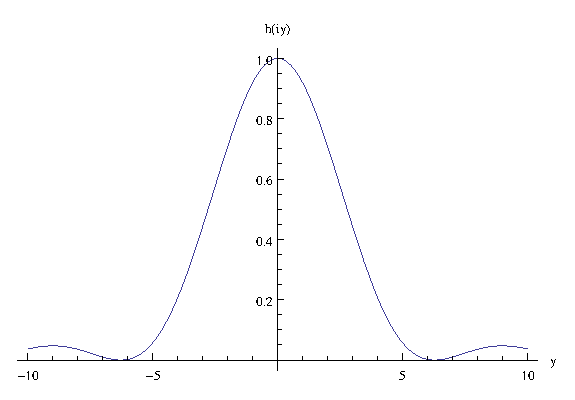
\includegraphics[width=0.65\textwidth]{./2_analysis/proof.eps}
\end{center}
\caption{График для ${|h(iy)|}^2$ при $-10 \leq y \leq 10$}
\end{figure}

Таким образом,

\begin{equation}\label{eq:h2}
|H_2(iy)| \leq |y| \gamma \tau = |z| \gamma \tau
\end{equation}

Объединяя (\ref{eq:h1}) и (\ref{eq:h2}) и потребовав $\gamma \tau < 1$, получим

\begin{equation}
|H_2(z)| < |z| < |H_1(z)|
\end{equation}

на границе области $D$. Таким образом, выполнены все условия теоремы Руше и у $\phi(z)$ нет нулей в $D$.

Таким образом, $\gamma \tau < 1$ \--- достаточное условие устойчивости решений дифференциального уравнения с запаздыванием.

\begin{equation}
{T'}_{k}(t) + \gamma(k^2) T_k (t-\tau)=0
\end{equation}

Отметим, что сколь угодно бы малым не было $\tau>0$ всегда можно найти такой номер $k$, начиная с которого не выполняется достаточное условие сходимости $\gamma \tau < 1$.